\documentclass[12pt]{beamer}
\usepackage{cmap}
\usepackage[T2A]{fontenc}
\usepackage[utf8]{inputenc}
\usepackage{ifluatex}
\usefonttheme[onlymath]{serif}
\usepackage{svg}
\usepackage{enumerate}
\usepackage{hyperref}
\usepackage{mathtools}
\setbeamertemplate{footline}[frame number]
\definecolor{beamer@darkgreen}{rgb}{0,0.6,0}
\setbeamercolor{normal text}{fg=black,bg=white}
\setbeamercolor{title}{fg=black,bg=beamer@darkgreen}
\setbeamercolor{frametitle}{fg=black,bg=beamer@darkgreen}
\setbeamercolor{background canvas}{parent=normal text}

\usepackage[english,russian]{babel}
\usepackage{graphicx}
\usepackage{listings}
\DeclareMathOperator{\sign}{sign}

\usepackage{enumerate}

\author{Катя Тузова}
\title{Машинное обучение}
\date{}

\usepackage{gensymb}

\subtitle{Лекция 11. Нейронные сети.}

\begin{document}	
\frame{\titlepage}

\begin{frame}\frametitle{Разбор летучки}

\end{frame}

\begin{frame}\frametitle{Нейрон}
\begin{figure}[htbp]
  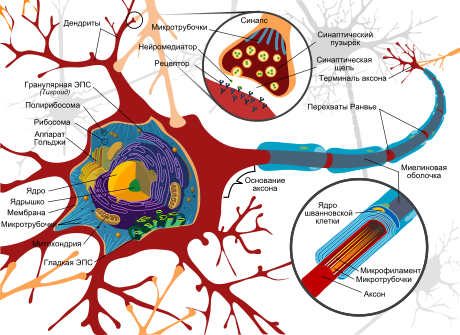
\includegraphics[height=200pt, keepaspectratio = true]{images/neuron}   
\end{figure}

\end{frame}


\begin{frame}\frametitle{Линейная модель нейрона}
Модель МакКаллока-Питтса:\\
$f_j: X \rightarrow R, j = 1,\dots, n$ — числовые признаки\\
$a(x,w) = \sigma(\langle w, x_i \rangle) = \sigma(\sum\limits_{j=1}^n w_j f_j(x) - w_0)$\\
где $w_0, w_1, \dots,w_n \in R$ -- веса признаков\\
$\sigma(s)$ -- функция активации (например, $\sign$)

\begin{figure}[htbp]
  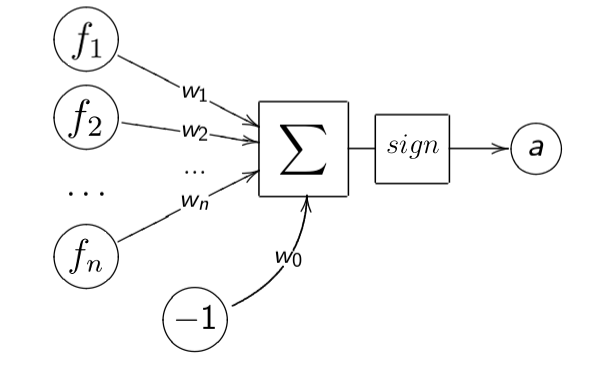
\includegraphics[height=100pt, keepaspectratio = true]{images/neuron-scheme}   
\end{figure}

\end{frame}

\begin{frame}\frametitle{Линейные алгоритмы классификации и регрессии}
Задача классификации: \\
$Y = \left\{ \pm1 \right\}, a(x,w) = \sign \langle w, x_i \rangle $\\
$Q(w;X^l) = \sum\limits_{i=1}^l \mathcal{L} \langle w, x_i\rangle y_i \rightarrow \min\limits_w$
Задача регрессии:\\
$Y = R, a(x,w) = \sigma(\langle w, x_i \rangle)$\\
$Q(w;X^l) = \sum\limits_{i=1}^l (\sigma(\langle w, x_i \rangle) - y_i)^2 \rightarrow \min\limits_w $
\end{frame}

\begin{frame}\frametitle{Нейронная реализация логических функций}

\begin{figure}[htbp]
  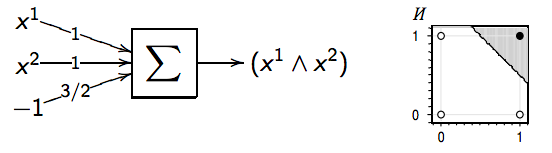
\includegraphics[height=60pt, keepaspectratio = true]{images/OR}   
\end{figure}

\begin{figure}[htbp]
  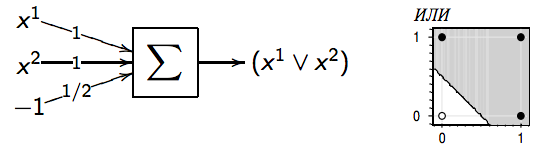
\includegraphics[height=60pt, keepaspectratio = true]{images/AND}   
\end{figure}

\end{frame}

\begin{frame}\frametitle{Нейронная реализация логических функций}
Функции И, ИЛИ, НЕ от бинарных переменных $x_1$ и $x_2$:\\
$$x_1 \wedge x_2 = x_1 + x_2 - \frac{3}{2} > 0$$\\
$$x_1 \vee x_2 = x_1 + x_2 - \frac{1}{2} > 0$$\\
$$\neg x_1 = -x_1 + \frac{1}{2}> 0$$
\end{frame}


\begin{frame}\frametitle{Логическая функция XOR}

\begin{figure}[htbp]
  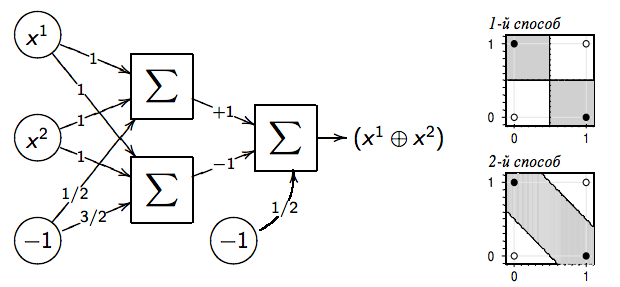
\includegraphics[height=150pt, keepaspectratio = true]{images/XOR}   
\end{figure}
\end{frame}

\begin{frame}\frametitle{Логическая функция XOR}
Функция $x_1 \oplus x_2 = [x_1 \neq x_2]$ не реализуема одним нейроном.\\
Два способа реализации:\\
\begin{enumerate}[--]
\item Добавлением нелинейного признака:\\
$x_1 \oplus x_2 = [x_1 + x_2 + 2x_1x_2 - \frac{1}{2} > 0]$
\item Сетью (двухслойной суперпозицией) функций И, ИЛИ, НЕ:\\
$x_1 \oplus x_2 = [(x_1 \vee x_2) - (x_1 \wedge x_2) - \frac{1}{2} > 0]$
\end{enumerate}
\end{frame}

\begin{frame}\frametitle{Любую ли функцию можно представить нейросетью?}
\begin{enumerate}[--]
\item Двухслойная сеть в $\left\{0, 1 \right\}^n$ позволяет реализовать произвольную булеву функцию.
\item Двухслойная сеть в $\mathbb{R}^n$ позволяет отделить произвольный выпуклый многогранник.
\item Трёхслойная сеть $\mathbb{R}^n$ позволяет отделить произвольную многогранную область, не обязательно выпуклую, и даже не обязательно связную.
\item С помощью линейных операций и одной нелинейной функции активации $\phi$ можно приблизить любую непрерывную функцию с любой желаемой точностью
\end{enumerate}
\end{frame}

\begin{frame}\frametitle{Практические рекомендации}
\begin{enumerate}[--]
\item Двух-трёх слоёв обычно достаточно.
\item Можно достраивать нейроны в произвольных местах сети по необходимости, вообще не заботясь о числе слоёв.
\end{enumerate}
\end{frame}

\begin{frame}\frametitle{Многослойная нейронная сеть}
Пусть для общности $Y = \mathbb{R}^M$, для простоты слоёв только два.\\

\begin{figure}[htbp]
  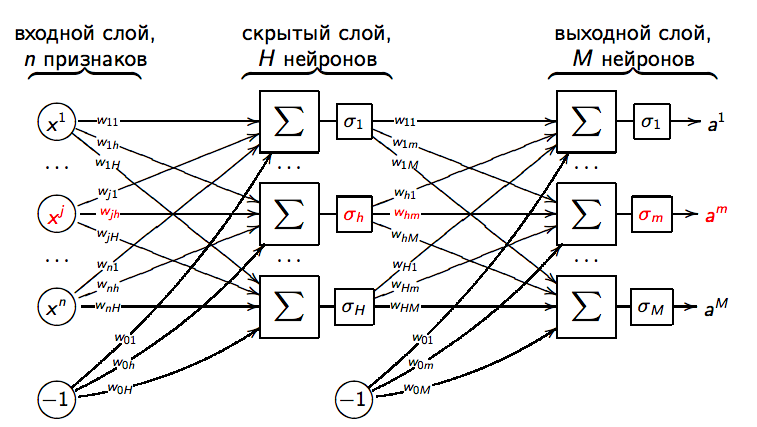
\includegraphics[height=150pt, keepaspectratio = true]{images/neural_network}   
\end{figure}
\end{frame}

\begin{frame}\frametitle{Стохастический градиент}
Задача минимизации суммарных потерь:\\
${Q}(\mathbf{w}) = \sum\limits_{i=1}^l \mathcal{L}(\langle \mathbf{w}, \mathbf{x_i} \rangle y_i) \rightarrow \min\limits_w$ \\
Input: $X^l$, $\alpha$, $\eta$\\
Output: $w_0, w_1, \dots, w_n$\\
\vspace{3mm}
Перемешать данные в $X^l$\\
Инициализировать: $w_j$, $j=0,\dots, n$\\
\hspace{35mm} ${Q}(\mathbf{w}) = \sum\limits_{i=1}^l \mathcal{L}(\langle \mathbf{w}, \mathbf{x_i} \rangle y_i)$\\
Повторить пока $Q$ и/или $w$ не стабилизируются:\\
\hspace{5mm} Взять $x_i$ из $X^l$\\
\hspace{5mm} Потеря: $\varepsilon_i = \mathcal{L}(\langle \mathbf{w}, \mathbf{x_i} \rangle y_i)$\\
\hspace{5mm} Градиентный шаг: $w =  w - \alpha \mathcal{L}'(\langle \mathbf{w}, \mathbf{x_i}\rangle y_i)\mathbf{x_i}y_i$\\
\hspace{5mm} Оценить $Q = (1-\eta)Q + \eta \varepsilon_i$
\end{frame}


\begin{frame}\frametitle{Задача дифференцирования суперпозиции функций}
Выходные значения сети $a^m(x_i)$, $m = 1,\dots,M$ на объекте $x_i$:\\
$$a^m(x_i) = \sigma_m (\sum\limits_{h=0}^H w_{hm} u^h(x_i)), \hspace{5mm} u^h(x_i) = \sigma_h (\sum\limits_{j=0}^J w_{jh} f_j(x_i))$$\\
Пусть для конкретности $\mathcal{L}_i(w)$ -- средний квадрат ошибки:\\
$$\mathcal{L}_i(w) = \frac{1}{2} \sum\limits_{m=1}^M (a^m(x_i) - y_i^m)^2$$\\
Промежуточная задача: найти частные производные\\
$$\frac {\partial \mathcal{L}_i(w)}{\partial a^m} \hspace{5mm} \frac {\partial \mathcal{L}_i(w)}{\partial u^h}$$
\end{frame}

\begin{frame}\frametitle{Быстрое вычисление градиента}
Промежуточная задача: частные производные\\
$$\frac{\partial \mathcal{L}_i(w)}{\partial a^m} = a^m (x_i) - y_i^m = \varepsilon^m_i$$ -- это ошибка на выходном слое\\
$$\frac{\partial \mathcal{L}_i(w)}{\partial u^h} = \sum\limits_{m=1}^M (a^m(x_i) - y_i^m) \sigma'_m w_{hm} = \sum\limits_{m=1}^M \varepsilon^m_i \sigma'_m w_{hm} = \varepsilon^h_i$$ -- назовём это ошибкой на выходном слое. \\
Похоже, что $\varepsilon_i^h$ вычисляется по $\varepsilon_i^m$, если запустить сеть «задом наперёд»:\\

\begin{figure}[htbp]
  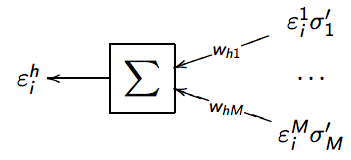
\includegraphics[height=50pt, keepaspectratio = true]{images/backpropagation}   
\end{figure}

\end{frame}

\begin{frame}\frametitle{Быстрое вычисление градиента}
Теперь, имея частные производные $\mathcal{L}_i(w)$ по $a^m$ и $u^h$, легко выписать градиент $\mathcal{L}_i(w)$ по весам $w$:\\
\vspace{5mm}
Вопрос: как?
\end{frame}

\begin{frame}\frametitle{Быстрое вычисление градиента}
Теперь, имея частные производные $\mathcal{L}_i(w)$ по $a^m$ и $u^h$, легко выписать градиент $\mathcal{L}_i(w)$ по весам $w$:\\

$$\frac {\partial \mathcal{L}_i(w)}{\partial w_{hm}} = \frac {\partial \mathcal{L}_i(w)}{\partial a^m} \frac {\partial a^m}{\partial w_{hm}} = \varepsilon^m_i \sigma'_m u^h()x_i, \hspace{2mm} m = 1,\dots,M, \hspace{2mm} h = 0,\dots, H$$\\

$$\frac {\partial \mathcal{L}_i(w)}{\partial w_{jh}} = \frac {\partial \mathcal{L}_i(w)}{\partial u^h} \frac {\partial u^h}{\partial w_{jh}} = \varepsilon_i^h \sigma'_h f_j(x_i), \hspace{2mm} h = 1,\dots,H, \hspace{2mm} j = 0,\dots, n$$ \\

\end{frame}


\begin{frame}\frametitle{Алгоритм обратного распространения ошибки}
Input: $X^l = (x_i, y_i)_{i=1}^l \subset \mathbb{R}^n \times \mathbb{R}^M$, $H$, $\lambda$, $\eta$\\
Output: синаптические веса $w_{jh}$, $w{hm}$\\
Повторять пока $Q$ не стабилизируется:\\
\hspace{5mm} выбрать объект $x_i$ из $X^l$\\
$\begin{cases}
\hspace{5mm} u^h_i = \sigma_h (\sum\limits_{j=0}^J w_{jh} x_i^j), \hspace{4mm} h = 1, \dots, H\\
\hspace{5mm} a^m_i = \sigma_m (\sum\limits_{h=0}^H w_{hm} u_i^h), \hspace{4mm} \varepsilon_i^m = a_i^m - y_i^m, \hspace{4mm} m = 1, \dots, M\\
\hspace{5mm} \mathcal{L} = \sum\limits_{m=1}^M (\varepsilon_i^m)^2\\
\end{cases}$\\
$\begin{cases} \hspace{5mm} \varepsilon_i^h = \sum\limits_{m=1}^M \varepsilon_i^m \sigma'_m w_{hm}, \hspace{4mm} h = 1, \dots, H\end{cases}$\\
$\begin{cases} \hspace{5mm} w_{hm} = w_{hm} - \eta \varepsilon_i^m \sigma'_m u_i^h, \hspace{4mm} h = 0, \dots, H, \hspace{4mm} m = 1, \dots, M\\
\hspace{5mm} w_{jh} = w_{jh} - \eta \varepsilon_i^h \sigma'_h x_i^j, \hspace{4mm} j = 0, \dots, n, \hspace{4mm} h = 1, \dots, H\\
\hspace{5mm} Q = (1 - \lambda)Q + \lambda \mathcal{L}\end{cases}$\\
\end{frame}

\begin{frame}\frametitle{Особенности}
\begin{enumerate}[+]
\item Эффективность: градиент вычисляется за время, сравнимое со временем вычисления самой сети
\item Легко обобщается на любые $\sigma$, $\mathcal{L}$
\item Возможно динамическое (потоковое) обучение
\item На сверхбольших выборках не обязательно брать все $x_i$
\item возможность распараллеливания
\end{enumerate}

\begin{enumerate}[--]
\item возможна медленная сходимость
\item застревание в локальных минимумах
\item проблема переобучения
\item подбор комплекса эвристик является искусством
\end{enumerate}
\end{frame}


\begin{frame}\frametitle{Стандартные эвристики для метода SG}
Применимы все те же эвристики, что и в обычном SG.\\

Напомните.
\end{frame}

\begin{frame}\frametitle{Стандартные эвристики для метода SG}
\begin{enumerate}[--]
\item Инициализация весов
\item Порядок предъявления объектов
\item Оптимизация величины градиентного шага
\item Регуляризация (сокращение весов)
\end{enumerate}
\end{frame}

\begin{frame}\frametitle{Новые проблемы}
\begin{enumerate}[--]
\item Выбор функций активации в каждом нейроне
\item Выбор числа слоёв и числа нейронов;
\item Выбор значимых связей;
\end{enumerate}
\end{frame}

\begin{frame}\frametitle{Ускорение сходимости}
\begin{enumerate}[--]
\item Тщательный подбор начального приближения
\item Выбивание из локальных минимумов
\item Адаптивный градиентный шаг
\item Метод сопряжённых градиентов и chunking -- разбиение суммы $Q(w) = \sum\limits_{i=1}^l \mathcal{L}_(w)$ на блоки
\end{enumerate}
\end{frame}

\begin{frame}\frametitle{Начальное приближение}
Нейроны настраиваются как отдельные линейные алгоритмы:
\begin{enumerate}[--]
\item либо по случайной подвыборке $X' \subseteq X^l$
\item либо по случайному подмножеству входов
\item либо из различных случайных начальных приближений
\end{enumerate}
Tем самым обеспечивается различность нейронов.
\end{frame}

\begin{frame}\frametitle{Улучшение сходимости}
Левенберга-Марквардта
TODO
\end{frame}

\begin{frame}\frametitle{Оптимизация структуры сети}
Динамическое наращивание сети.\\
\begin{enumerate}[--]
\item Обучение при заведомо недостаточном числе нейронов $H$
\item После стабилизации  $Q(w)$ -- добавление нового нейрона и его инициализация путём обучения
\item Снова итерации BackProp
\end{enumerate}

Инициализация нового нейрона:\\
\begin{enumerate}[--]
\item либо по случайной подвыборке $X' \subset X$
\item либо по объектам с наибольшими значениями потерь
\item либо по случайному подмножеству входов
\item либо из различных случайных начальных приближений
\end{enumerate}

\end{frame}

\begin{frame}\frametitle{Оптимизация структуры сети}
Прореживание сети.\\
TODO
\end{frame}


\begin{frame}\frametitle{Специальные нейронные сети}
TODO
% сверточные

\end{frame}

\begin{frame}\frametitle{На следующей лекции}
\begin{itemize}
\item[--] 
\end{itemize}
\end{frame}
\end{document}
